\chapter{Figures and Tables\label{chap:figsandtabs}}

\lipsum[41]
A two-dimensional model of aspect\index{a}{aspect} is provided in
Figure~\ref{fig:2d}.

\lipsum[42]

\begin{figure}[h]
	\centering\label{fig:2d}
	\begin{tikzpicture}
	  \draw[thick] (0,0) --++(0,-3) --++(3,0);
	  \draw (0,-0.5) node[left] {{\em q}};
	  \draw (2.5,-3) node[below] {{\em t}};
	  \draw (-0.5,-2) node[left] {{\em rest state}};
	  \draw (-0.5,-1) node[left] {{\em crying}};
	  \draw[thick, dashed, KUCrimson] (0,-2) --++(1,0);
	  \draw[thick, dashed, KUCrimson] (2,-2) --++(1,0);
	  \draw[thick, KUCrimson] (1,-2) --++(0,1);
	  \draw[thick, KUCrimson] (2,-1) --++(0,-1);
	  \draw[thick, KUCrimson, decorate, decoration=snake]
	  (1,-1) --++(1,0);
	  %\draw[thick, KUCrimson] (1,-2) --++(0,.5) --++(.25,.6) --++(.25,-.6) --++(.25,.6) --++(.25,-.6) --++(0,-.5);
	\end{tikzpicture}
	\caption[The Russian delimitative in two dimensions]{A two-dimensional
	  model of the Russian delimitative \cite[79--80]{Croft:2012aa}.}
\end{figure}

\lipsum[43-46]
Results from three different machine learning models is provided in
Table~\ref{tab:ml}.

\lipsum[47]

\begin{table}[h]
	\centering\label{tab:ml}
	\caption{Accuracy of machine learning models}\vspace{1ex}
	\begin{tabular}{@{}llll@{}}
	 & {\bf Model 1} & {\bf Model 2} & {\bf Model 3} \\
	 & Decision Tree (J48) & Logistic Regression & Random Forest \\ \midrule
	 Training error & 0.0744 & 0.0691 & 0.0754 \\
	 Standard deviation & 0.2217 & 0.2595 & 0.1677 \\
	 Correctly Classified Instances & 946 & 931 & 963 \\
	\end{tabular}
\end{table}

\lipsum[48-52]

\begin{figure}[h]
	\centering\label{fig:photo}
	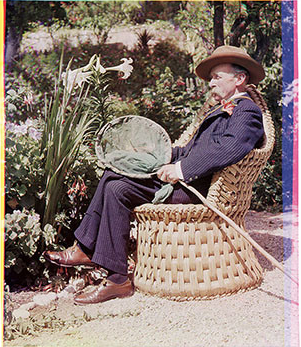
\includegraphics{../graphics/Acland1903.png}
	\caption[A public-domain photograph]{A photograph in the public domain.}
\end{figure}

\lipsum[53-56]
